\chapter{Architecture Constraints}

\section{Environment}
\label{sec:Environment}
In the context of an AUTOSAR ECU, RTA-SUM modules are technically built as Application Software Components. Therefore, each RTA-SUM module requires a full AUTOSAR SW stack to run. We assume that the following AUTOSAR SW will be used:
\input{generated/tables/tools.tex}

\section{Layers Definition}
The SUM\_SrvcMgr is a software module in the application layer of the standardized architecture of AUTOSAR (Figure~\ref{fig:Layers}). 
It interacts with other RTA-SUM modules, with external SWCs and with components of the BSW. In the last two cases, the RTE is the means through which the interaction takes place.
\begin{figure}[htp]
\centering
	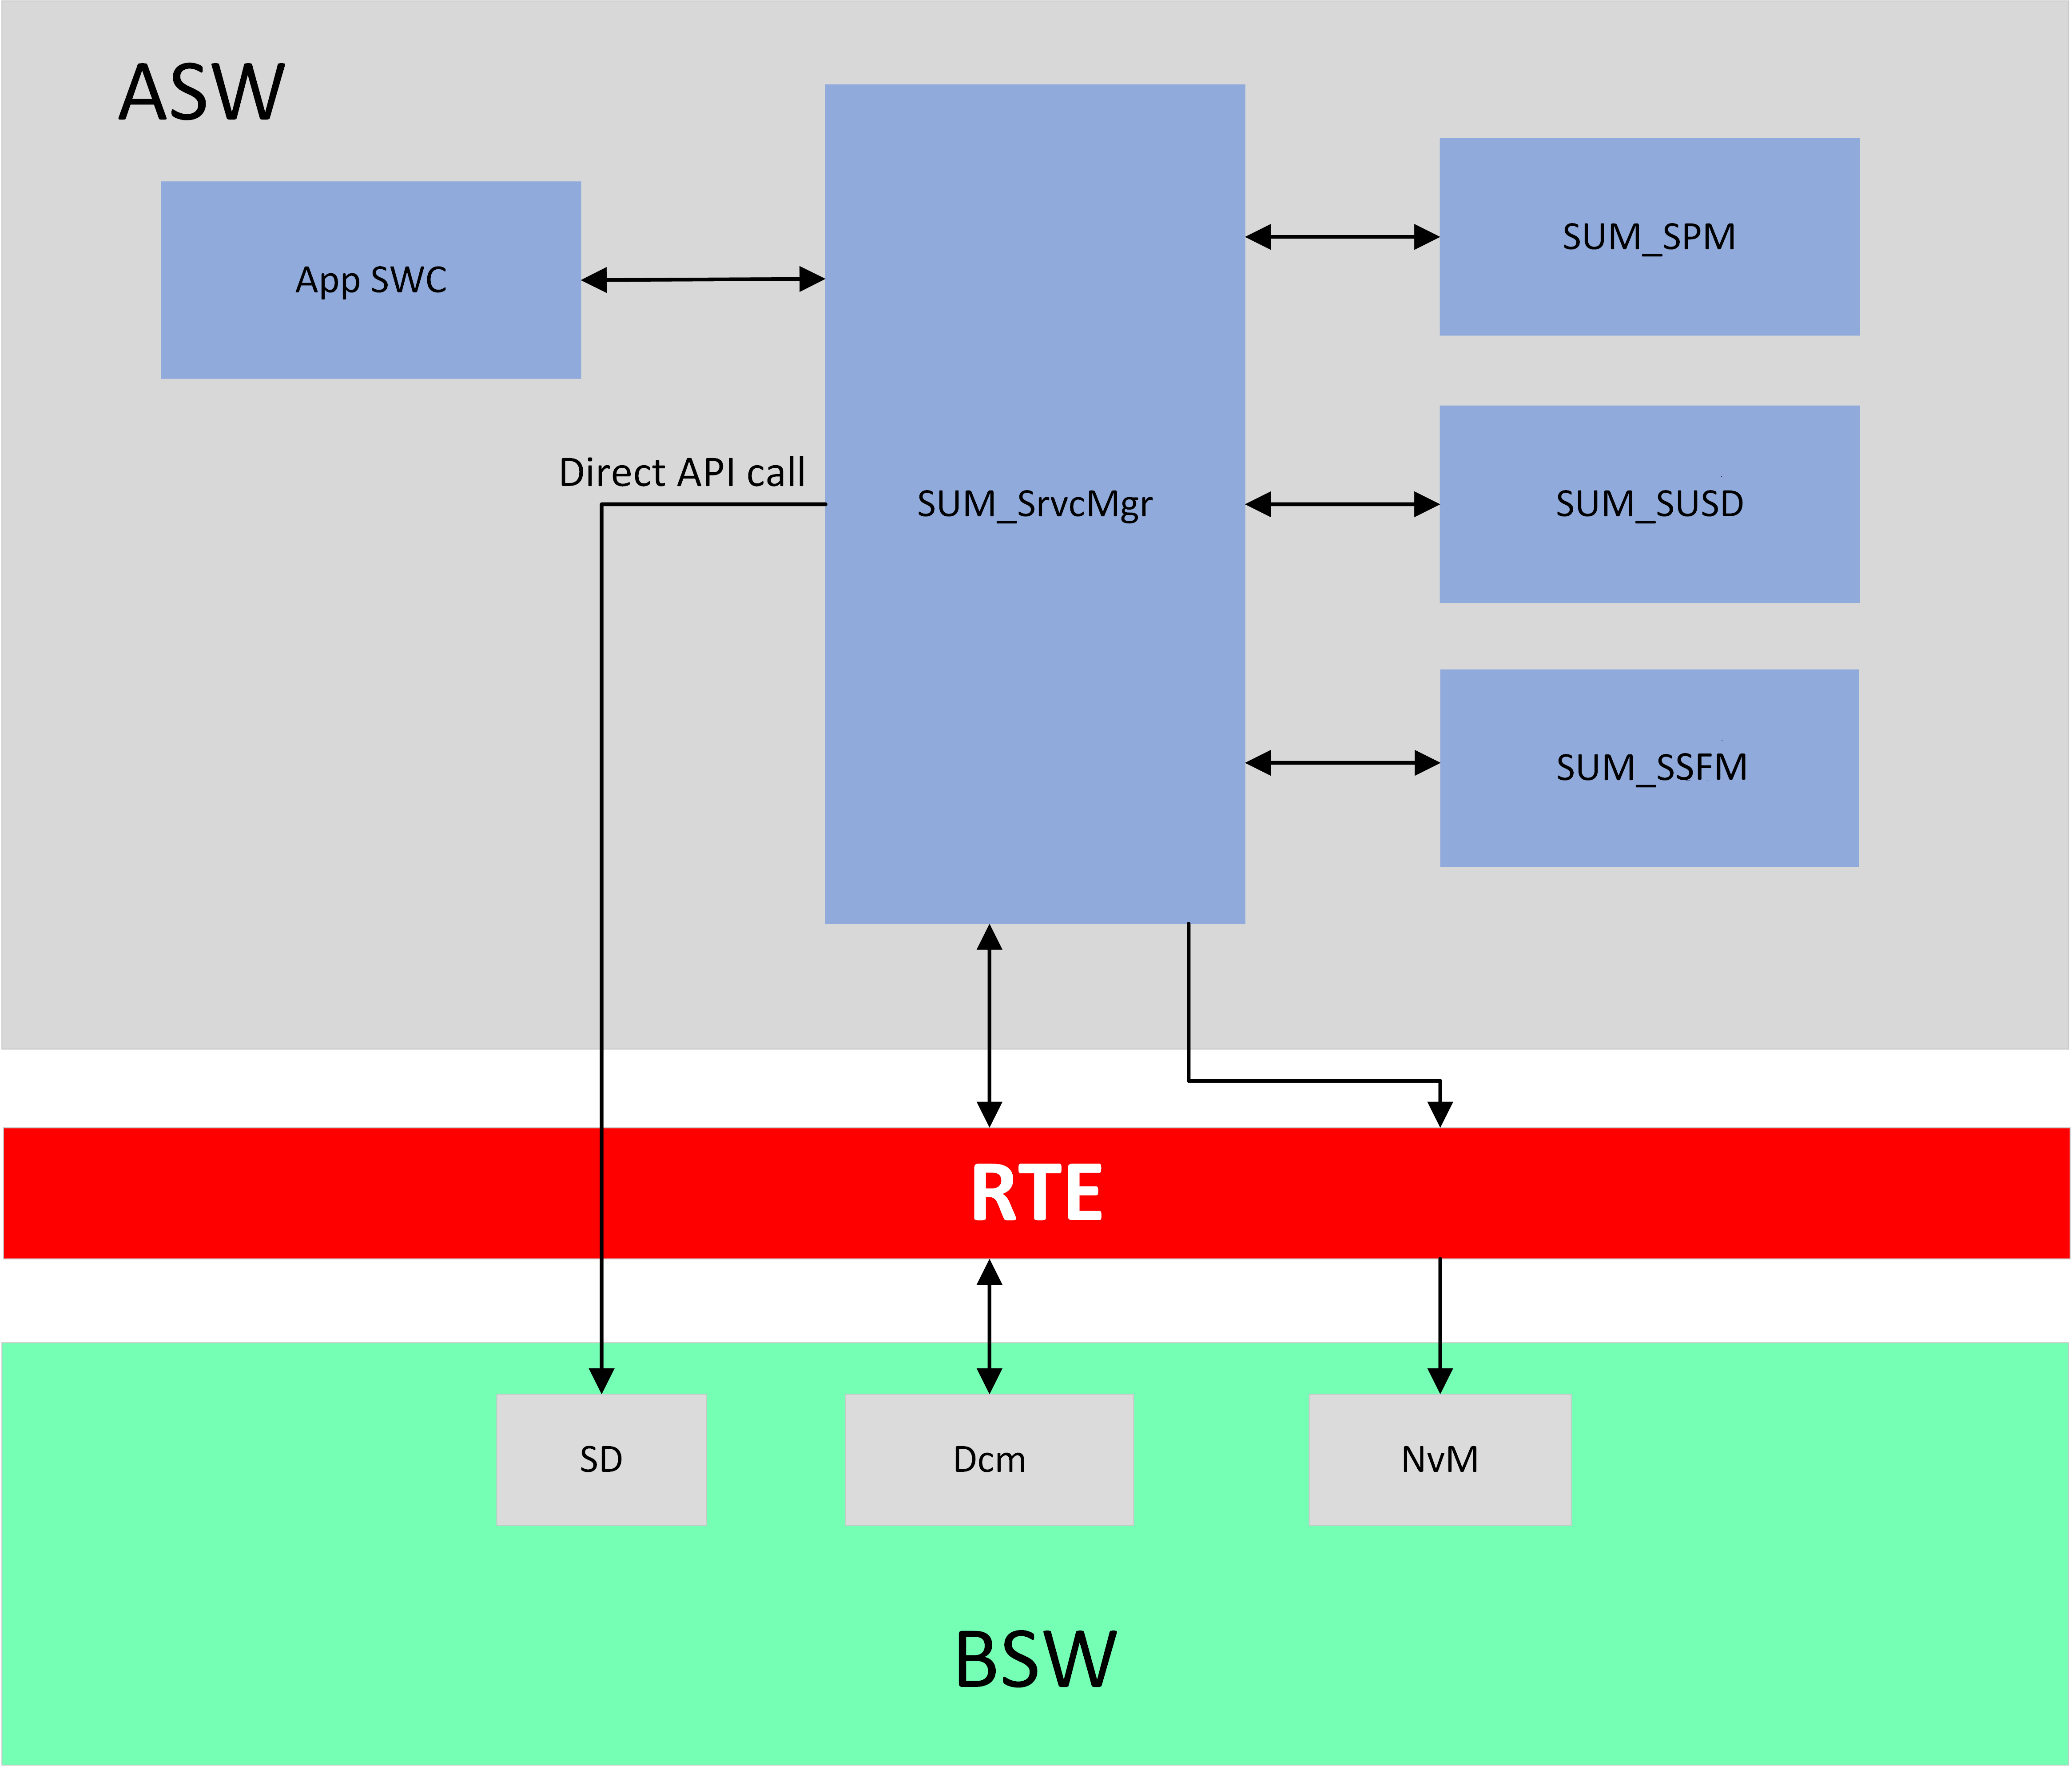
\includegraphics[scale=0.5]{images/SrvcMgr_System_Block_View.png}
	\caption{System layer overview.}
	\label{fig:Layers}
\end{figure}

\section{Generic component interface}

The external interfaces of SUM\_SrvcMgr, and most of the interactions among SUM modules are specified in GM SDV-8201.

Section \ref{sec:portInterfaces} reports all interfaces that are implemented on RTA-SUM SrvcMgr ports to the RTE.

\section{Other constraints and assumptions}
SrvcMgr has service needs that are provided by the AUTOSAR BSW. For an ECU to implement SrvcMgr, the following must be true:

\begin{itemize}
\item The ECU must have an RTE that supports:
  \begin{itemize}
  \item Sender / Receiver and Client /Server port interface
  \end{itemize}
\item The ECU must have AUTOSAR SD module
\item The ECU must have AUTOSAR NvM module
\item The ECU must have AUTOSAR Dcm module
\item It is assumed that the ECU initialization sequence is designed such that any NVM needed for the SrvcMgr function is available prior to SrvcMgr being initialized.
\item SrvcMgr shall be initialized after the Sd module to assure proper behavior on service handling.
\end{itemize}
